\documentclass[a4paper, 11pt]{article}

\usepackage[a4paper,margin=1in]{geometry}
\usepackage[english]{babel}
\usepackage[utf8]{inputenc}
\usepackage[T1]{fontenc}
\usepackage{lmodern}
\usepackage{listings}
\usepackage{graphicx}
\usepackage{amsmath}
\usepackage{amssymb}
\usepackage{amsthm}
\usepackage{framed}
\usepackage{amsfonts}
\usepackage{caption}
\usepackage{subcaption}
\usepackage{listings}
\usepackage{centernot}
\usepackage{dirtytalk}
\usepackage{relsize}
\usepackage{color}
\usepackage[dvipsnames]{xcolor}
\usepackage{fancyhdr}
\usepackage{lastpage}
\usepackage{algorithm}
\usepackage{setspace}
\usepackage[noend]{algpseudocode}

\graphicspath{{../imgs/}}

\definecolor{morange}{RGB}{237,106,90}
\definecolor{mgreen}{RGB}{63,127,95}
\definecolor{mpurple}{RGB}{127,0,85}

\lstset{
  basicstyle=\small\ttfamily, % Global Code Style
  captionpos=b, % Position of the Caption (t for top, b for bottom)
  extendedchars=true, % Allows 256 instead of 128 ASCII characters
  tabsize=2, % number of spaces indented when discovering a tab
  columns=fixed, % make all characters equal width
  keepspaces=true, % does not ignore spaces to fit width, convert tabs to spaces
  showstringspaces=false, % lets spaces in strings appear as real spaces
  breaklines=true, % wrap lines if they don't fit
  frame=trbl, % draw a frame at the top, right, left and bottom of the listing
  frameround=tttt, % make the frame round at all four corners
  framesep=4pt, % quarter circle size of the round corners
  numbers=left, % show line numbers at the left
  numberstyle=\tiny\ttfamily, % style of the line numbers
  commentstyle=\color{mgreen}, % style of comments
  keywordstyle=\color{mpurple}, % style of keywords
  stringstyle=\color{morange}, % style of strings
}

% TAILLE DES PAGES (A4 serré)

\setlength{\parindent}{0pt}
\setlength{\parskip}{1em}
%% \setlength{\textwidth}{17cm}
%% \setlength{\textheight}{24cm}
%% \setlength{\oddsidemargin}{-.7cm}
%% \setlength{\evensidemargin}{-.7cm}
%% \setlength{\topmargin}{-.5in}


\pagestyle{fancy}
\renewcommand{\arraystretch}{1.4}
\renewcommand{\headrulewidth}{0pt}
\renewcommand{\footrulewidth}{0.6pt}% default is 0pt
\lhead{}
\rhead{}
\lfoot{Page \thepage\ of \pageref{LastPage}}
\rfoot{Rémi Lespinet}
\cfoot{}
\cfoot{}


\newtheorem{lemma}{Lemma}[section]

\newcounter{cquestion}[subsection]
\renewcommand{\thecquestion}{\arabic{cquestion}}
\newenvironment{question}
{\par \vspace{0.5em} \noindent \stepcounter{cquestion} \hspace{-1em}
  \textbf{\thecquestion.}}
{}

\newcounter{csubquestion}[cquestion]
\renewcommand{\thecsubquestion}{\alph{csubquestion}}
\newenvironment{subquestion}
{\par \vspace{0.5em} \noindent \stepcounter{csubquestion} \hspace{-1em}
  \textbf{(\thecsubquestion)}}
{}

\newenvironment{note}
{\begin{framed} \textbf{Note : }}
  {\end{framed}}

% Commandes de mise en page
\newcommand{\file}[1]{\emph{#1}}
\newcommand{\name}[1]{\emph{#1}}

\newcommand{\pfigref}[1]{(Figure \ref{#1} p. \pageref{#1})}
\newcommand{\ptableref}[1]{(Table \ref{#1} p. \pageref{#1})}
\newcommand{\peqref}[1]{(\ref{#1} p. \pageref{#1})}

\newcommand{\figref}[1]{(Figure \ref{#1})}
\newcommand{\tableref}[1]{(Table \ref{#1})}

\newcommand{\itemi}{\item[$\bullet$]}
% Commandes color
\newcommand{\colgood}[1]{\color{ForestGreen} #1}
\newcommand{\colbad}[1]{\color{BrickRed} #1}


% Commandes de maths
\newcommand{\function}[3]{#1 : #2 \to #3}
\newcommand{\intn}[2]{\left\{ #1 \dots #2 \right\}}
\newcommand{\intr}[2]{\left[ #1 ; #2 \right]}
\newcommand{\intro}[2]{\left] #1 ; #2 \right[}
\newcommand{\dotp}[2]{\langle #1, #2 \rangle}
\newcommand{\logn}[1]{\ln\left( #1\right)}
%% \newcommand{\det}[1]{\left| #1 \right|}
\newcommand{\pd}[2]{\frac{\partial #1}{\partial #2}}
\newcommand{\norm}[1]{\|#1\|}
\newcommand{\set}[2]{\left\{ #1 \hspace{.5em} ; \hspace{.5em}#2 \right\}}
\newcommand{\tr}[1]{\text{Tr}\left( #1 \right)}

\newcommand{\bigCI}{\mathrel{\text{\scalebox{1.07}{$\perp\mkern-10mu\perp$}}}}
\newcommand{\nbigCI}{\centernot{\bigCI}}
\newcommand{\indep}[2]{#1 \bigCI #2}
\newcommand{\nindep}[2]{#1 \nbigCI #2}
\newcommand{\indepcond}[3]{#1 \bigCI #2 \hspace{.5em} | \hspace{.5em} #3 }
\newcommand{\nindepcond}[3]{#1 \nbigCI #2 \hspace{.5em} | \hspace{.5em} #3 }
\newcommand{\pcond}[2]{p(#1 \hspace{-.2em}\mid\hspace{-.2em} #2)}
\newcommand{\parampcond}[3]{p_{#1}(#2 \hspace{-.2em}\mid\hspace{-.2em} #3)}
\newcommand{\kldiv}[2]{D( #1 \| #2)} % Kullback-Leibler divergence
\newcommand{\ex}[1]{\mathbb{E}\left[ #1 \right]} % Expectation
\newcommand{\excond}[2]{\mathbb{E}\left[ #1 \hspace{-.2em}\mid\hspace{-.2em} #2\right]}
\newcommand{\paramexcond}[3]{\mathbb{E}_{#1}\left[ #2 \hspace{-.2em}\mid\hspace{-.2em} #3\right]}
\newcommand{\grad}[1]{\nabla{#1}}
\newcommand{\paramgrad}[2]{\nabla_{#1}{#2}}

\newcommand{\iid}{i.i.d }
\newcommand{\wrt}{w.r.t }

% Commandes informatique
\newcommand{\pfun}[1]{{\textbf{\texttt{#1}}}}

\newcommand{\ipart}[1]{\vspace{0.5em}\textbf{#1}\vspace{0.5em}}

\newcommand{\bigsum}{\mathlarger{\sum}}
\newcommand{\Bigsum}{\mathlarger{\bigsum}}

\pagenumbering{arabic}

\title{\textsc{Graphical models - MVA 2017/2018 \\ \emph{Homework 3}} }
\author{Rémi Lespinet}
\date{}

\begin{document}

\maketitle
\thispagestyle{fancy}

\section{HMM Implementation}

The HMM model that we use in this homework is represented in the
figure \ref{fig:hmm}.

\begin{figure}[h!]
  \centering
  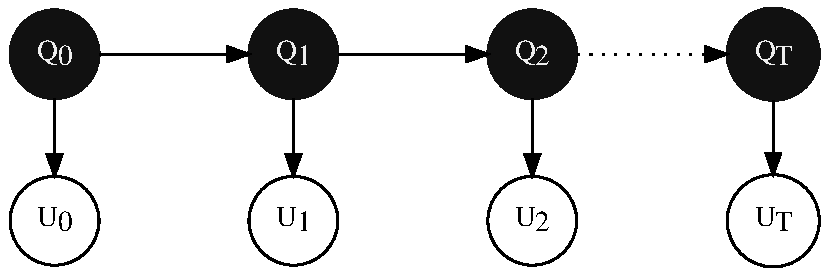
\includegraphics[width=0.5\textwidth]{hmm.pdf}
  \caption{Representation of the HMM model}\label{fig:hmm}
\end{figure}

\begin{question}
  \ipart{Recurence formulas}

  With these notations, the alpha-beta recursion formulas are given by
  \begin{displaymath}
    \left\{
      \begin{array}{ll}
        % \alpha_t (q_t) = \mu_{u_t \to z_t}(z_t) \mu_{z_{t-1} \to z_t}(z_t) \\
        \alpha_0(q_0) &= \pcond{u_0}{q_0} p(q_0) \\
        \alpha_{t+1} (q_{t+1}) &= \pcond{\overline{u_{t+1}}}{q_{t+1}} \sum_{q_t} \pcond{q_{t+1}}{q_t} \alpha_t(q_t) \\
      \end{array}
    \right.
  \end{displaymath}
  and
  \begin{displaymath}
    \left\{
      \begin{array}{ll}
        \beta_T(q_T) &= 1 \\
        \beta_{t}(q_t) &= \sum_{q_{t+1}} \pcond{q_{t+1}}{q_t}\pcond{\overline{u_{t+1}}}{q_{t+1}} \beta_{t+1}(q_{t+1})
      \end{array}
    \right.
  \end{displaymath}
  % In our example we consider a HMM with gaussian emission (independant
  % from $t$), hence
  % \begin{displaymath}
  %   \pcond{u_t}{q_t} = \dfrac{1}{\sqrt{(2\pi)^d\det{\Sigma_{q_t}}}} \exp{\left( - \dfrac{1}{2} (u_t - \mu_{q_t})^T \Sigma_{q_t}^{-1} (u_t - \mu_{q_t})^T \right)}
  % \end{displaymath}

  \ipart{Log-coding}

  In the computation, we use the log coding which is given by the
  formulas
  \begin{displaymath}
    \log \alpha_{t+1}(q_{t+1}) =
    \log{\pcond{\overline{u_{t+1}}}{q_{t+1}}} +
    \log{\sum_{q_t} \exp{\Big( \log{\pcond{q_{t+1}}{q_t}} + \log{\alpha_t(q_t)}\Big)}}
  \end{displaymath}
  and
  \begin{displaymath}
    \log{\beta_{t}(q_t)} =
    \log{\sum_{q_{t+1}} \exp{ \Big(
        \log{\pcond{q_{t+1}}{q_t}} +
        \log{\pcond{\overline{u_{t+1}}}{q_{t+1}}} +
        \log{\beta_{t+1}(q_{t+1})}
        \Big) }}
  \end{displaymath}
  And we use that
  \begin{displaymath}
    \log{\sum_{i = 1}^n \exp{\left( x_i\right)}} = a + \log{\sum_{i = 1}^n \exp{\left( x_i - a\right)}}
  \end{displaymath}
  with
  \begin{displaymath}
    a = \max_{i = 1, \dots, n} x_i
  \end{displaymath}
  (This is done in the \verb+log_sum_exp+ function)

  We can then compute
  \begin{displaymath}
    \log{p(u_0 \dots u_T)} = \log{\sum_{q_t} \exp{\left(\log \alpha_t(q_t) + \log \beta_t(q_t)\right)}}
  \end{displaymath}
  and
  \begin{displaymath}
    \begin{split}
      \log{\gamma_t(q_t)}
      = & \log{\pcond{q_t}{u_0, \dots u_T}} \\
      = & \log{\left( \dfrac{\alpha_t(q_t) \beta_t(q_t)}{p(u_0 \dots u_T)} \right)} \\
      = & \log{ \alpha_t(q_t) } + \log{\beta_t(q_t)} - \log{p(u_0 \dots u_T)} \\
    \end{split}
  \end{displaymath}
  finally,
  \begin{displaymath}
    \begin{split}
      \log{\xi_{t, t+1}(q_t)}
      = & \log{\pcond{q_{t+1}, q_t}{u_0, \dots u_T}} \\
      = & \log{\left( \dfrac{\alpha_t(q_t) \beta_{t+1}(q_{t+1}) \pcond{q_{t+1}}{q_t} \pcond{u_{t+1}}{q_{t+1}}}{p(u_0 \dots u_T)} \right)} \\
      = &\log{\alpha_t(q_t)} + \log{\beta_{t+1}(q_{t+1})} + \log{\pcond{q_{t+1}}{q_t}} \\
      + & \log{\pcond{u_{t+1}}{q_{t+1}}} - \log{p(u_0 \dots u_T)} \\
    \end{split}
  \end{displaymath}


\end{question}

\begin{question}
  In this question, we are using the same parameters for the means and
  covariances of the Gaussians as the one obtained Homework 2 i.e.
  The table \ref{tab:parameters-hw2} summarize the values of the
  parameters. These parameters are also represented in figure
  \ref{fig:clustering-notrain}.

  \begin{table}[h!]
    \centering
    \begin{tabular}{| l | c | c | c | c |}
      \hline
      & Gaussian 0 & Gaussian 1 & Gaussian 2 & Gaussian 3 \\
      \hline
      means
      & $\mu_0 = \begin{pmatrix} 3.80 \\ -3.80 \end{pmatrix}$
      & $\mu_1 = \begin{pmatrix} 3.98 \\  3.77 \end{pmatrix}$
      & $\mu_2 = \begin{pmatrix} 3.06 \\ -3.53  \end{pmatrix}$
      & $\mu_3 = \begin{pmatrix} 2.03 \\  4.17 \end{pmatrix}$ \\
      \hline
      cov.
      & $\Sigma_0 = \begin{pmatrix}
        0.92  &  0.06 \\
        0.06 &  1.87
      \end{pmatrix}$
                   & $\Sigma_1 = \begin{pmatrix}
                     0.21 &  0.29 \\
                     0.29 & 12.24
                   \end{pmatrix}$
                   & $\Sigma_2 = \begin{pmatrix}
                     6.24 &  6.05 \\
                     6.05  &  6.18
                   \end{pmatrix}$
                   & $\Sigma_3 = \begin{pmatrix}
                     2.90 &  0.21 \\
                     0.21 &  2.76
                   \end{pmatrix}$ \\
      \hline
    \end{tabular}
    \captionof{table}{Parameters learnt by Expectation Maximization on
      Gaussian mixtures in previous homework for the same
      dataset} \label{tab:parameters-hw2}
  \end{table}

  \begin{figure}[h!]
    \centering
    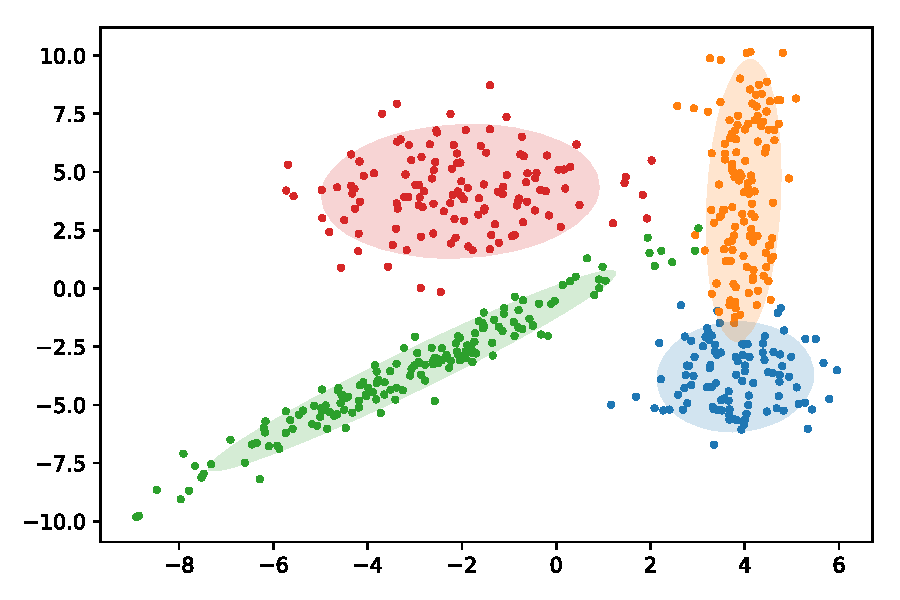
\includegraphics[width=0.7\textwidth]{clustering_notrain.pdf}
    \caption{Representation of the means and covariances learnt by
      Expectation Maximization on a Gaussian mixture (4 kernels) in
      the previous homework for the same dataset (Ellipses contain
      95\% of the distributions)}\label{fig:clustering-notrain}
  \end{figure}

  The first $100$ points of $\pcond{q_t}{u_0 \dots u_T}$ are
  represented in figure \ref{fig:filtering-notrain}. Even if have
  taken a relatively uniform transition probability matrix (the
  probabilities, $\pcond{q_{t+1} = i}{q_t = j}$ are equals given
  $i \ne j$), we see some patterns in the data, which make us believe
  that the data has probably been generated with a HMM (in which case
  we see that the probability of staying in state 2 seems to be high,
  the probability of reaching state 3 from state 1 also seem to be
  high (and conversely))

  \begin{figure}[h!]
    \centering
    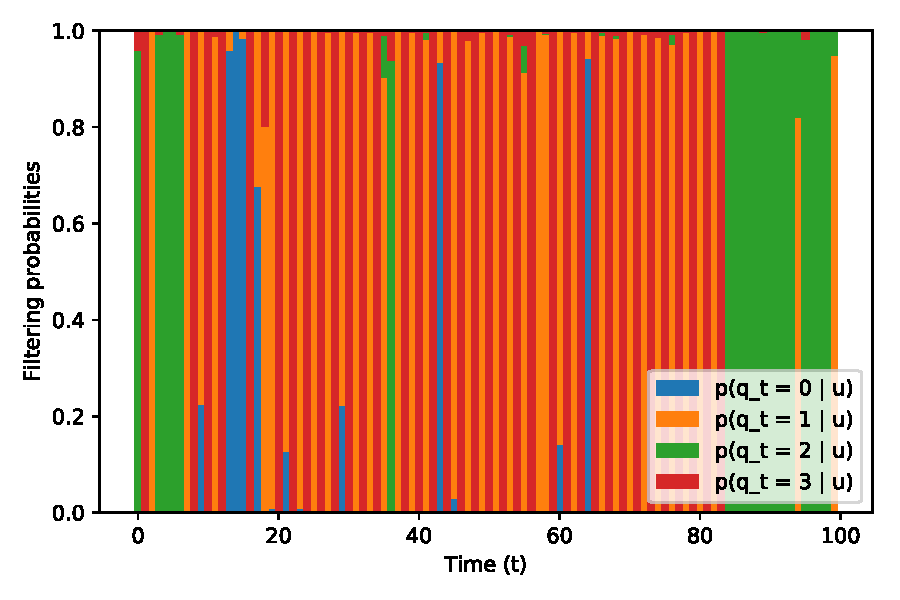
\includegraphics[width=0.7\textwidth]{filtering_notrain.pdf}
    \caption{Representation of the filtering probabilities
      $\pcond{q_t}{u_0, \dots u_T}$ for each state for the HMM with
      chosen parameters (not trained)}\label{fig:filtering-notrain}
  \end{figure}

\end{question}

\newpage
\begin{question}
  Let us consider the case where each $q_t$ take $M$ values.
  The parameters of the model are
  \begin{displaymath}
    \theta = (\pi, A, \mu_0, \Sigma_0, \dots \mu_M, \Sigma_M)
  \end{displaymath}
  We have
  \begin{displaymath}
    p_\theta(q, y) = % p_\theta(q_0, \dots q_T, u_0, \dots u_T) =
    p_\theta(q_0)
    \prod_{t = 0}^{T-1} \parampcond{\theta}{q_{t+1}}{q_t}
    \prod_{t = 0}^{T} \parampcond{\theta}{u_{t}}{q_t}
  \end{displaymath}

  The complete log likelihood in the case of this HMM is expressed as
  \begin{displaymath}
    \mathcal{L}(\theta, q, y) =
    \log{p_\theta(q_0)} +
    \sum_{t = 0}^{T-1} \log{\parampcond{\theta}{q_{t+1}}{q_t}} +
    \sum_{t = 0}^{T} \log{\parampcond{\theta}{u_{t}}{q_t}}
  \end{displaymath}

  Using the one hot encoding
  \begin{displaymath}
    q_{t}^{i} =
    \left\{
      \begin{array}{ll}
        1 & \text{ if } q_t = i \\
        0 & \text{ otherwise }  \\
      \end{array}
    \right.
  \end{displaymath}
  We can rewrite the first term as
  \begin{align*}
    \log{p_\theta(q_0)}
    = \log{\pi(q_0)}
    = \log{\prod_{i = 1}^M \pi_i^{q_0^i}}
    = \sum_{i = 1}^M q_0^i \log{\pi_i}
  \end{align*}
  The second term can be simplified as
  \begin{align*}
    \log{\parampcond{\theta}{q_{t+1}}{q_t}}
    = \log{a_ {q_{t}, q_{t+1}}}
    = \log{\prod_{i, j = 1}^M a_{i,j}^{q_{t}^{i} q_{t+1}^{j}}}
    = \sum_{i, j = 1}^M q_{t}^{i} q_{t+1}^{j} \log{a_{i, j}}
  \end{align*}
  Finally, we have
  % \begin{displaymath}
  %   \parampcond{\theta}{u_{t}}{q_t} = \dfrac{1}{\sqrt{(2\pi)^d\det{\Sigma_{q_t}}}} \exp{\left( - \dfrac{1}{2} (u_t - \mu_{q_t})^T \Sigma_{q_t}^{-1} (u_t - \mu_{q_t})^T \right)}
  % \end{displaymath}
  \begin{displaymath}
    \log{\parampcond{\theta}{u_{t}}{q_t}} % = - \dfrac{1}{2} \log{\left((2\pi)^d\det{\Sigma_{q_t}}\right)} - \dfrac{1}{2} (u_t - \mu_{q_t})^T \Sigma_{q_t}^{-1} (u_t - \mu_{q_t})^T
    = - \dfrac{1}{2} \log{(2\pi)^d} - \dfrac{1}{2}\log{\det{\Sigma_{q_t}}} - \dfrac{1}{2} (u_t - \mu_{q_t})^T \Sigma_{q_t}^{-1} (u_t - \mu_{q_t})^T
  \end{displaymath}
  Which can also be rewriten using the one hot encoding as
  \begin{equation}
    \log{\parampcond{\theta}{u_{t}}{q_t}} = - \dfrac{1}{2} \log{(2\pi)^d} - \dfrac{1}{2} \sum_{i = 1}^M q_t^i \log{\det{\Sigma_{i}}} - \dfrac{1}{2} \sum_{i = 1}^M q_t^i (u_t - \mu_{i})^T \Sigma_{i}^{-1} (u_t - \mu_{i})^T
  \end{equation}
  Hence, the complete log likelihood is given by
  \begin{framed}
    \begin{displaymath}
      \begin{split}
        \mathcal{L}(\theta, q, y)
        &= \sum_{i = 1}^M q_0^i\log{\pi_i} + \sum_{t = 0}^{T-1} \sum_{i, j = 1}^M q_{t}^{i} q_{t+1}^{j} \log{a_{i, j}} \\
        &- \dfrac{1}{2} \log{(2\pi)^d} - \dfrac{1}{2} \sum_{t=0}^T\sum_{i = 1}^M q_t^i \log{\det{\Sigma_{i}}} - \dfrac{1}{2} \sum_{t=0}^T \sum_{i = 1}^M q_t^i (u_t - \mu_{i})^T \Sigma_{i}^{-1} (u_t - \mu_{i})^T
      \end{split}
    \end{displaymath}
  \end{framed}

  \ipart{E step}

  Taking the same notation as in the polycopié, we write
  \begin{displaymath}
    \gamma_{t}^{i} \triangleq \pcond{q_t = i}{u_0, \dots u_T}
  \end{displaymath}
  and
  \begin{displaymath}
    \xi_{t, t+1}^{i, j} \triangleq \pcond{q_t = i, q_{t+1} = j}{u_0, \dots u_T}
  \end{displaymath}

  We then compute the following expectations
  \begin{align*}
    \paramexcond{q_0, \dots q_T}{q_t^i q_{t+1}^j}{u_0, \dots u_T}
    & = \sum_{q_t, q_{t+1}} q_t^i q_{t+1}^j \pcond{q_t, q_{t+1}}{u_0, \dots u_T} \\
    & = \pcond{q_t = i, q_{t+1} = j}{u_0, \dots, u_T} \\
    & = \xi_{t, t+1}^{i, j}
  \end{align*}
  And
  \begin{align*}
    \paramexcond{q_0, \dots q_T}{q_t^i}{u_0, \dots u_T}
    & = \sum_{q_t} q_t^i \pcond{q_t}{u_0, \dots u_T} \\
    & = \pcond{q_t = i}{u_0, \dots, u_T} \\
    & = \gamma_t^i
  \end{align*}
  We can then write the expected complete log likelihood

  \begin{displaymath}
    \begin{split}
      \paramexcond{q_0, \dots q_T}{\mathcal{L}(\theta ; q, y)}{u_0, \dots u_T}
      &= \sum_{i = 1}^M \gamma_0^i\log{\pi_i} + \sum_{t = 0}^{T-1} \sum_{i, j = 1}^M \xi_{t, t+1}^{i, j} \log{a_{i, j}} \\
      &- \dfrac{1}{2} \log{(2\pi)^d} - \dfrac{1}{2} \sum_{t=0}^T\sum_{i = 1}^M \gamma_t^i \log{\det{\Sigma_{i}}} \\
      &- \dfrac{1}{2} \sum_{t=0}^T \sum_{i = 1}^M \gamma_t^i (u_t - \mu_{i})^T \Sigma_{i}^{-1} (u_t - \mu_{i})
    \end{split}
  \end{displaymath}

  \ipart{M step}

  Looking at the expression of the expected complete log-likelihood, we
  see that we can minimize separately over $\pi$, $(a_{i, j})$ and
  $(u_i, \Sigma_i)$

  \ipart{Maximizing over $\pi$}

  We want to maximize
  \begin{equation*}
    \begin{aligned}
      & \text{maximize}
      & & \sum_{i = 1}^M \gamma_0^i \log{\pi_i} \\
      & \text{subject to}
      & & \pi_1 + \dots + \pi_M = 1
    \end{aligned}
  \end{equation*}

  The Lagrangian is
  \begin{displaymath}
    \mathcal{L}(\pi, \lambda) = \sum_{i = 1}^M \gamma_0^i \log{\pi_i} - \lambda \left(\sum_{i = 1}^M{\pi_i} - 1\right)
  \end{displaymath}

  This is a concave problem (as a non negative weighted sum of concave
  functions), we have feasibility (there is no inequatity
  constraints), hence by Slater constraint qualification strong
  duality holds. The KKT conditions are

  \begin{displaymath}
    \left\{
    \begin{array}{l}
      \forall i \in \intn{1}{M},\ \dfrac{\gamma_0^i}{\pi_i} - \lambda = 0 \\
      \pi_0 + \dots + \pi_M = 1
    \end{array}
    \right.
  \end{displaymath}

  Posing
  \begin{displaymath}
    \hat{\pi}_i = \dfrac{\gamma_0^i}{\sum_{i = 1}^M {\gamma_0^i}}
  \end{displaymath}
  and
  \begin{displaymath}
    \hat{\lambda} = \sum_{i = 1}^M {\gamma_0^i}
  \end{displaymath}
  we see that the couple $(\hat{\pi}, \hat{\lambda})$ verify the KKT
  conditions and is thus primal-dual optimal. Since
  \begin{displaymath}
    \sum_{i = 1}^M \gamma_0^i = \sum_{i = 1}^M \pcond{q_t = i}{u_0, \dots u_T} = 1
  \end{displaymath}
  We finally obtain
  \begin{framed}
    \begin{displaymath}
      \hat{\pi}_i = \gamma_0^i
    \end{displaymath}
  \end{framed}


  \ipart{Maximizing over A}

  We want to maximize
  \begin{equation*}
    \begin{aligned}
      & \text{maximize}
      & & \sum_{t = 0}^{T-1} \sum_{i, j = 1}^M \xi_{t, t+1}^{i, j} \log{a_{i, j}} \\
      & \text{subject to}
      & & a_{i, 1} + \dots + a_{i, M} = 1,\ i = 1 \dots M
    \end{aligned}
  \end{equation*}

  The lagrangian is
  \begin{displaymath}
    \mathcal{L}(\pi, \lambda) =
    \sum_{t = 0}^{T-1} \sum_{i, j = 1}^M \xi_{t, t+1}^{i, j} \log{a_{i, j}} -
    \sum_{i = 1}^M \lambda_i \left( \sum_{j = 1}^M a_{i, j} - 1 \right)
  \end{displaymath}

  This is also a concave problem (for the same reasons), it is also
  feasible, hence by Slater constraint qualification strong duality
  holds. The KKT conditions are

  \begin{displaymath}
    \left\{
    \begin{array}{l}
      \displaystyle
      \forall i, j \in \intn{1}{M},\ \sum_{t = 0}^{T-1} \dfrac{\xi_{t, t+1}^{i, j}}{a_{i, j}} - \lambda_i = 0 \\
      \forall i \in \intn{1}{M},\ a_{i, 1} + \dots + a_{i, M} = 1
    \end{array}
    \right.
  \end{displaymath}

  % \begin{displaymath}
  %   \left\{
  %   \begin{array}{cl}
  %     \displaystyle
  %     \sum_{t = 0}^{T-1} \dfrac{\xi_{t, t+1}^{i, j}}{a_{i, j}} + \lambda_i & i, j = 1 \dots a \\
  %     M_{i, 1} + \dots + a_{i, M} = 1 & i = 1 \dots M
  %   \end{array}
  %   \right.
  % \end{displaymath}
  Summing the first condition on the row, we obtain
  \begin{displaymath}
    \sum_{t = 0}^{T-1} \sum_{j = 1}^M \xi_{t, t+1}^{i, j} - \sum_{j = 1}^M a_{i,j}\lambda_i = 0
  \end{displaymath}
  Using the second condition, we have
  \begin{displaymath}
    \lambda_i = \sum_{t = 0}^{T-1} \sum_{j = 1}^M \xi_{t, t+1}^{i, j}
  \end{displaymath}
  Thus,
  \begin{framed}
    \begin{displaymath}
      a_{i,j} = \dfrac{\sum_{t = 0}^{T-1} \xi_{t, t+1}^{i, j}}{\sum_{j = 1}^M \sum_{t = 0}^{T-1} \xi_{t, t+1}^{i, j}}
    \end{displaymath}
  \end{framed}

  \ipart{Maximizing over $(\mu_i, \Sigma_i)$}

  The optimization problem that we want to solve is
  \begin{equation*}
    \begin{aligned}
      & \text{maximize}
      & &  - \sum_{t=0}^T\sum_{i = 1}^M \gamma_t^i \log{\det{\Sigma_{i}}} - \sum_{t=0}^T \sum_{i = 1}^M \gamma_t^i (u_t - \mu_{i})^T \Sigma_{i}^{-1} (u_t - \mu_{i}) \\
    \end{aligned}
  \end{equation*}

  Let $\Omega = \Sigma^{-1}$, because
  \begin{displaymath}
    \begin{array}{clc}
      \mathcal{S}_n^{++} & \to & \mathcal{S}_n^{++} \\
      X & \to & X^{-1} \\
    \end{array}
  \end{displaymath}
  is one-to-one with image covering $\mathbb{S}_n^{++}$ (set of
  positive semi-definite matrices), we can solve the following
  optimization problem
  \begin{equation*}
    \begin{aligned}
      & \text{maximize}
      & &  \sum_{t=0}^T\sum_{i = 1}^M \gamma_t^i \log{\det{\Omega_{i}}} - \sum_{t=0}^T \sum_{i = 1}^M \gamma_t^i (u_t - \mu_{i})^T \Omega_{i} (u_t - \mu_{i}) \\
    \end{aligned}
  \end{equation*}
  and a solution $(\mu_i, \Omega_i)$ to this problem obtains a
  solution to the original problem :
  $(\mu_i, \Omega_i^{-1})$. With this change of variable
  the objective function is now concave ($X \to \log\det(X)$ is
  concave) and $X \to a^T X b$ is linear.

  We can minimize \wrt $\mu_i$ first, this is a concave function of
  $\mu_i$ (covariance matrix is symmetric positive semidefinite, and so
  is it's inverse) taking the gradient leads to
  \begin{displaymath}
    -2 \sum_{t = 0}^{T} \gamma_t^i \Omega_i (u_t - \mu_i) = 0
  \end{displaymath}
  Hence, assuming that the covariance matrix is definite,
  \begin{displaymath}
     \sum_{t = 0}^{T} \gamma_t^i \mu_i = \sum_{t = 0}^{T} \gamma_t^i u_t
  \end{displaymath}
  and
  \begin{framed}
    \begin{displaymath}
      \mu_i = \dfrac{\sum_{t = 0}^{T} \gamma_t^i u_t}{\sum_{t = 0}^{T} \gamma_t^i}
    \end{displaymath}
  \end{framed}
  Which is simply the average of the observations $u_t$ such that $q_t = i$.
  We can now derive with respect to $\Omega_i$. First, we notice that
  \begin{align*}
    \sum_{t=0}^T \sum_{i = 1}^M \gamma_t^i (u_t - \mu_{i})^T \Omega_{i} (u_t - \mu_{i})
    & = \sum_{t=0}^T \sum_{i = 1}^M \gamma_t^i \tr{(u_t - \mu_{i})^T \Omega_{i} (u_t - \mu_{i})} \\
    & = \sum_{t=0}^T \sum_{i = 1}^M \gamma_t^i \tr{\Omega_{i} (u_t - \mu_{i}) (u_t - \mu_{i})^T}
  \end{align*}
  Hence setting the gradient to $0$,
  \begin{displaymath}
    \sum_{t=0}^T \gamma_t^i \Omega_{i}^{-1} - \sum_{t=0}^T \gamma_t^i (u_t - \mu_{i}) (u_t - \mu_{i})^T = 0
  \end{displaymath}
  Hence,
  \begin{displaymath}
    \Omega_{i}^{-1} = \dfrac{\sum_{t=0}^T \gamma_t^i (u_t - \mu_{i}) (u_t - \mu_{i})^T}{\sum_{t=0}^T \gamma_t^i }
  \end{displaymath}
  And
  \begin{framed}
    \begin{displaymath}
      \Sigma_{i} = \dfrac{\sum_{t=0}^T \gamma_t^i (u_t - \mu_{i}) (u_t - \mu_{i})^T}{\sum_{t=0}^T \gamma_t^i }
    \end{displaymath}
  \end{framed}


\end{question}

\begin{question}
  The initial transition matrix and initial probability distribution
  are uniform, the parameters of the gaussian emission kernels have
  been initialized with the values obtained in the previous homework.
  The table \ref{tab:parameters-train} summarize the values of
  parameters ($\mu_i, \Sigma_i$) learned by the EM algorithm.  The
  table \ref{tab:transition-train} represents the obtained transition
  matrix. As we expected in our discussion on figure
  \ref{fig:filtering-notrain}, we see that the probability $A_{1, 3}$,
  $A_{3, 1}$ and $A_{2, 2}$ (indicing the from $0$) are very high
  which means that their corresponding probabilities
  $\pcond{q_{t+1} = 1}{q_t = 3}$, $\pcond{q_{t+1} = 3}{q_t = 1$},
  $\pcond{q_{t+1} = 2}{q_t = 2$} are high. This means that the HMM
  successfuly learned the patterns that we observed (which correspond
  to the transition probabilities of the HMM that generated the data).

  \begin{table}[h!]
    \centering
    \begin{tabular}{| l | c | c | c | c |}
      \hline
      & Gaussian 0 & Gaussian 1 & Gaussian 2 & Gaussian 3 \\
      \hline
      means
      & $\mu_0 = \begin{pmatrix}  3.79 \\ -3.97 \end{pmatrix}$
      & $\mu_1 = \begin{pmatrix}  3.99 \\  3.63 \end{pmatrix}$
      & $\mu_2 = \begin{pmatrix} -2.97 \\ -3.45  \end{pmatrix}$
      & $\mu_3 = \begin{pmatrix} -1.95 \\  4.19  \end{pmatrix}$ \\
      \hline
      cov.
      & $\Sigma_0 = \begin{pmatrix}
        0.94 &  0.06 \\
        0.06 &  1.55
      \end{pmatrix}$
                   & $\Sigma_1 = \begin{pmatrix}
                     0.20 &  0.26 \\
                     0.26 & 12.34
                   \end{pmatrix}$
                   & $\Sigma_2 = \begin{pmatrix}
                     6.81 &  6.59 \\
                     6.59 &  6.69
                   \end{pmatrix}$
                   & $\Sigma_3 = \begin{pmatrix}
                     3.28 &  0.30  \\
                     0.30 &   2.83
                   \end{pmatrix}$ \\
      \hline
    \end{tabular}
    \captionof{table}{Parameters learned by Expectation Maximization on
      the HMM (on the train dataset) initialized with the values
      obtained in the previous homework} \label{tab:parameters-train}
  \end{table}

  \begin{table}[h!]
    \centering
    \begin{displaymath}
      A =
      \begin{pmatrix}
        0.88 &  0.05 &  0.03 &  0.04 \\
        0.01 &  0.02 &  0.03 &  0.93 \\
        0.02 &  0.07 &  0.90 &  0.01 \\
        0.05 &  0.87 &  0.06 &  0.02 \\
      \end{pmatrix}
    \end{displaymath}

    \captionof{table}{Transition matrix learned by Expectation Maximization on
      the HMM (on the train dataset)} \label{tab:transition-train}
  \end{table}

% initial probability :
% [[ 0.87859234  0.04762886  0.03420622  0.03957258]
%  [ 0.01209136  0.02246886  0.03264008  0.9327997 ]
%  [ 0.02011068  0.07245662  0.90067642  0.00675628]
%  [ 0.04635766  0.87485905  0.06301847  0.01576482]]
\end{question}

\begin{question}
  The incomplete log likelihood $p_\theta(u_0, \dots u_T)$ for the
  test and train data as a function of the iterations of the EM
  algorithm are given in the figure
  \ref{fig:log-likelihood-comparison}.  The algorithm stops when the
  variation of the incomplete log likelihood is below a threshold
  $\epsilon$ (in this case $\epsilon = 10^{-6}$). We notice that the
  algorithm converges in about 10 iterations in both cases (the
  initialization was very good). We also notice that the parameters
  learned are almost the same in both cases and that the likelihood
  obtained is very close. This means that they have probably been
  generated by the same HMM.

  % the HMM with parameters learnt from the EM algorithm on the training
  % data is more likely to generate this sequence of data than is the HMM
  \begin{figure}[h!]
    \centering
    \begin{subfigure}[t]{0.49\textwidth}
      \centering
      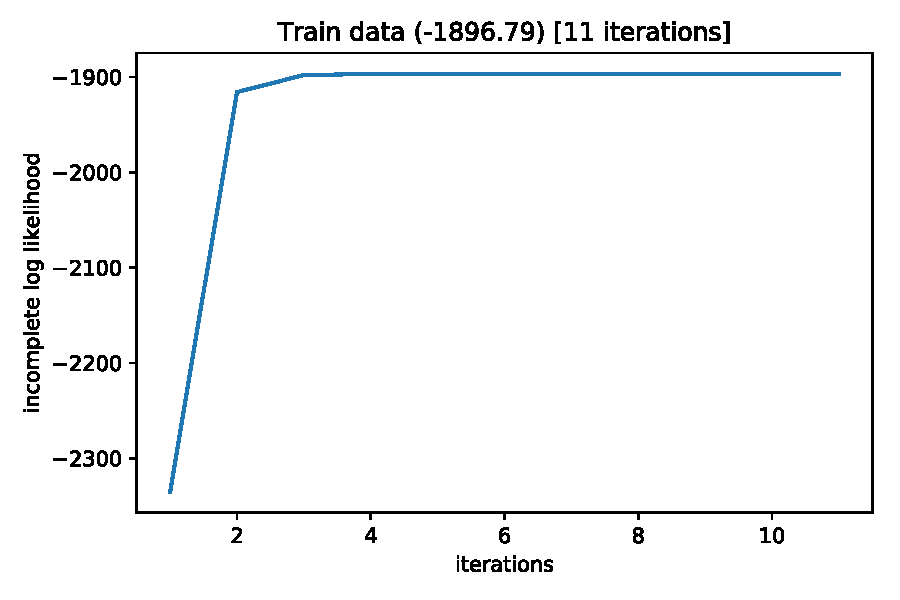
\includegraphics[width=\textwidth]{likelihood_train.pdf}
      \caption{Train data (500 points)}\label{fig:}
    \end{subfigure}
    \begin{subfigure}[t]{0.49\textwidth}
      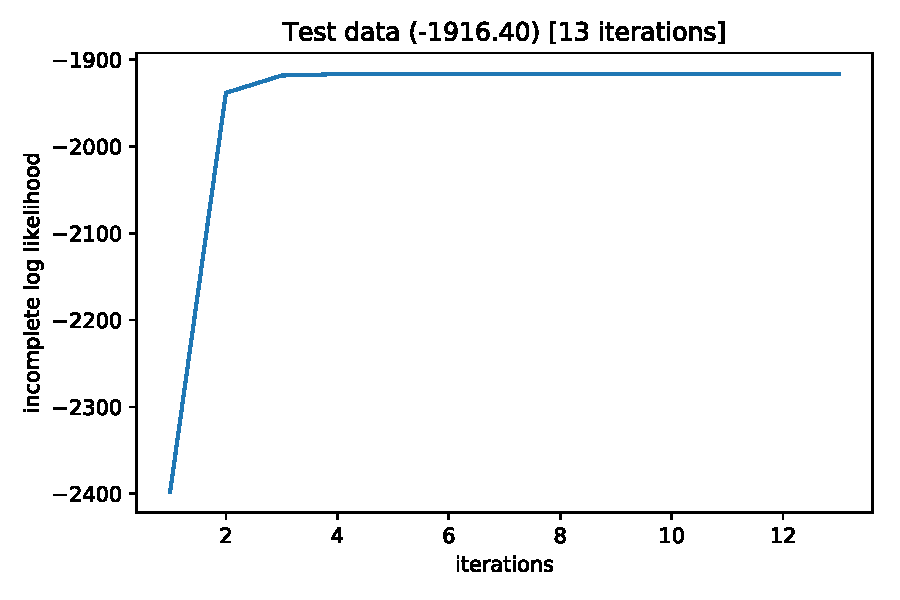
\includegraphics[width=\textwidth]{likelihood_test.pdf}
      \caption{Test data (500 points)}\label{fig:LDA-A-test}
    \end{subfigure}
    \caption{Evolution of the incomplete log likelihood for the
      train and test data with the number of iteration of the EM algorithm
    }\label{fig:log-likelihood-comparison}
  \end{figure}

\end{question}

\begin{question}
  The table \ref{tab:likelihood-comparison} compares the incomplete
  log likelihood obtained on the train and test dataset for the HMM
  (after EM parameter learning) with the different models of the
  previous homework (Isotropic and full GMM after EM learning).

  It makes sense to compare these models, because they all are
  expressing the incomplete log likelihood which can be viewed
  as the probability of observing these data given the model.

  As already explained in the previous homework, it makes sense that
  the likelihood of the Full GMM is higher than the Isotropic GMM,
  because the Isotropic GMM is a particular case of the Full GMM
  (where the covariances matrices can be written $\sigma_i I$) and
  hence by learning on the Full GMM, we are maximizing on a larger set.

  The exact same argument applies for the HMM and the Full GMM, the
  Full GMM is the particular case of a HMM whose transition matrix can
  be written as
  \begin{equation}
    \label{eq:no-transition}\tag{$\star$}
    A =
    \begin{pmatrix}
      \pi_0 & \pi_1 & \pi_2 & \pi_3 \\
      \pi_0 & \pi_1 & \pi_2 & \pi_3 \\
      \pi_0 & \pi_1 & \pi_2 & \pi_3 \\
      \pi_0 & \pi_1 & \pi_2 & \pi_3 \\
    \end{pmatrix}
  \end{equation}
  Which means that the probability of the next state does not depend
  on the probability of the current state.

  \begin{table}[h!]
    \centering
    \begin{tabular}{|l||c|c|}
      \hline
      & \textbf{Train} & \textbf{Test} \\
      \hline
      Isotropic GMM & -2652.89 & -2654.39 \\
      \hline
      Full GMM & -2332.29 & -2417.30 \\
      \hline
      HMM & -1896.79 & -1916.40\\
      \hline
    \end{tabular}
    \captionof{table}{Incomplete log likelihood of the train and test
      dataset obtained for different
      models} \label{tab:likelihood-comparison}
  \end{table}

\end{question}

\begin{question}
  For the studied HMM, the Viterbi algorithm aims to compute
  \begin{displaymath}
    \max_{q_0 \dots q_T}{\pcond{q_0 \dots q_T}{u_0, \dots u_T}}
  \end{displaymath}
  This is the same as maximizing
  \begin{displaymath}
    \max_{q_0 \dots q_T}{p(q_0 \dots q_T, \overline{u_0}, \dots \overline{u_T})}
  \end{displaymath}

  This can be rewriten as
  \begin{displaymath}
    \max_{q_0 \dots q_T}{\left(
        p(q_0) \prod_{t = 0}^T\pcond{\overline{u_t}}{q_t} \prod_{t=0}^{T - 1} \pcond{q_{t+1}}{q_t}
      \right)}
  \end{displaymath}

  \ipart{Algorithm derived from the book}

  This can be expanded to
  \begin{displaymath}
    \max_{q_T} \dots
    \max_{q_1} \Big( \pcond{q_2}{q_1} \pcond{\overline{u_1}}{q_1}
    \max_{q_0} \Big( p(q_0) \pcond{\overline{u_0}}{q_0} \pcond{q_1}{q_0} \Big) \Big)
  \end{displaymath}
  Let
  \begin{displaymath}
    m_1(q_1) = \max_{q_0} \Big( p(q_0) \pcond{\overline{u_0}}{q_0} \pcond{q_1}{q_0} \Big)
  \end{displaymath}
  We can then rewrite the previous formula :
  \begin{displaymath}
    \max_{q_T} \dots
    \max_{q_1} \Big( \pcond{q_2}{q_1} \pcond{\overline{u_1}}{q_1} m_1(q_1) \Big)
  \end{displaymath}
  This leads to the following recurrence formula
  \begin{framed}
    \begin{displaymath}
      \left\{
        \begin{array}{l}
          m_0(q_0)  = \pi(q_0) \\
          m_{t+1}(q_{t+1}) = \max_{q_{t}} \Big(
          \pcond{\overline{u_t}}{q_t} \pcond{q_{t+1}}{q_{t}} m_{t}(q_{t})
          \Big)
        \end{array}
      \right.
    \end{displaymath}
  \end{framed}

  % \begin{displaymath}
  %   p(q_0) \prod_{k = 0}^t\pcond{\overline{u_k}}{q_k} \prod_{k=0}^{t - 1} \pcond{q_{k+1}}{q_k}
  %   = \Big(p(q_0) \prod_{k = 0}^{t-1}\pcond{\overline{u_k}}{q_k} \prod_{k=0}^{t - 2} \pcond{q_{k+1}}{q_k}\Big)
  %   \pcond{\overline{u_t}}{q_t} \pcond{q_t}{q_{t-1}}
  % \end{displaymath}



  % \begin{displaymath}
  %   m_t(i) = \max_{q_0 \dots q_{t-1}}{p(q_0 \dots q_t = i, \overline{u_0}, \dots \overline{u_t})}
  % \end{displaymath}
  % Since $(q_0, \dots q_{t-1})$ and $(u_0, \dots u_{t-1})$ also form a

  % \begin{displaymath}
  %   m_t(i) = \max_{q_0 \dots q_{t-1}}{p(q_0 \dots q_t = i, \overline{u_0}, \dots \overline{u_t})}
  % \end{displaymath}





  % This is the same as maximizing
  % \begin{displaymath}
  %   \max_{q_0 \dots q_T}{p(q_0 \dots q_T, \overline{u_0}, \dots \overline{u_T})}
  % \end{displaymath}
  % Which can be rewriten as
  % \begin{displaymath}
  %   \max_{q_0 \dots q_T}{\left(
  %       p(q_0) \prod_{t = 0}^T\pcond{\overline{u_t}}{q_t} \prod_{t=0}^{T - 1} \pcond{q_{t+1}}{q_t}
  %     \right)}
  % \end{displaymath}
  % We can write this as
  % \begin{displaymath}
  %   \max_{q_T} \pcond{\overline{u_T}}{q_T} \max_{q_{T-1}} \pcond{q_{T}}{q_{T-1}} \max_{q_{T-2} \dots q_0}
  %   p(q_0) \prod_{t = 0}^{T-1}\pcond{\overline{u_t}}{q_t} \prod_{t=0}^{T - 2} \pcond{q_{t+1}}{q_t}
  % \end{displaymath}





  % \begin{displaymath}
  %   \max_{q_T} \dots
  %   \max_{q_1} \Big( \pcond{q_2}{q_1} \pcond{\overline{u_1}}{q_1}
  %   \max_{q_0} \Big( p(q_0) \pcond{\overline{u_0}}{q_0} \pcond{q_1}{q_0} \Big) \Big)
  % \end{displaymath}
  % Let
  % \begin{displaymath}
  %   m_1(q_1) = \max_{q_0} \Big( p(q_0) \pcond{\overline{u_0}}{q_0} \pcond{q_1}{q_0} \Big)
  % \end{displaymath}
  % We can rewrite the preceding term as
  % \begin{displaymath}
  %   \max_{q_T} \dots
  %   \max_{q_1} \Big( \pcond{q_2}{q_1} \pcond{\overline{u_1}}{q_1} m_1(q_1) \Big)
  % \end{displaymath}

  % Now, we want to compute the combination
  % $(\hat{q}_0, \dots \hat{q}_T)$ that realizes this maximum.  We can
  % easily get $q_T$

  % Suppose
  % that we know the value of a state $\hat{q}_t$ such that
  % $p(q_0, \dots, q_t = \hat{q}_t, u_0, u_t)$ realizes a maximum. Then we would know
  % that
  % \begin{displaymath}
  %   \hat{q}_{t-1} = \arg\max_{q_{t-1}} \Big( \pcond{\overline{u_t}}{q_t = \hat{q}_t} \pcond{q_t = \hat{q}_t}{q_{t-1}} T_{t-1}(q_{t-1}) \Big)
  % \end{displaymath}


  % leads to
  % \begin{displaymath}
  %   \max_{q_0 \dots q_T}{\pcond{q_0 \dots q_T}{u_0, \dots u_T}} =  \arg\max_{q_T} \pcond{\overline{u_T}}{q_T} m_{T}(q_T)
  % \end{displaymath}
  % Now we want to know the combination $(q_0, \dots q_T)$ such that
  % $\pcond{q_0 \dots q_T}{u_0, \dots u_T}$ realizes this maximum.

  % We already have
  % \begin{displaymath}
  %   \hat{q}_T = \arg\max_{q_T} \pcond{\overline{u_T}}{q_T} m_{T}(q_T)
  % \end{displaymath}

  At the end of the recurrence, we obtain
  \begin{displaymath}
    \max_{q_0 \dots q_T}{p(q_0 \dots q_T, \overline{u_0}, \dots \overline{u_T})}
    = \max_{q_T} \Big( m_{T-1}(q_T) \pcond{\overline{u_T}}{q_T} \Big)
  \end{displaymath}
  Now, we want to compute the combination
  $(\hat{q}_0, \dots \hat{q}_T)$ that realizes this maximum.  We can
  easily get a value for $\hat{q}_T$ by taking
  \begin{displaymath}
    \hat{q}_T = \arg\max_{q_T} \Big( m_{T-1}(q_T) \pcond{\overline{u_T}}{q_T} \Big)
  \end{displaymath}
  now that we have the value $\hat{q}_T$, we would like to know the
  value of all the states $\hat{q}_{t}$ that have been chosen to
  obtain the maximum value of
  $\max_{q_0 \dots q_T}{p(q_0 \dots q_T, \overline{u_0}, \dots
    \overline{u_T})}$. This can be easily computed at the forward pass
  using the following recurrence formula :
  \begin{displaymath}
    s_t(q_{t+1}) = \arg\max_{q_{t}} \Big(
    \pcond{\overline{u_t}}{q_t} \pcond{q_{t+1}}{q_{t}} m_{t}(q_{t})
    \Big)
  \end{displaymath}
  We can then determine $\hat{q}_t$ by simply computing
  $s_{t}(\hat{q}_{t+1})$.  The algorithm \ref{Viterbi} resumes these
  steps and traduce it for the case of a HMM with Gaussian emissions
  (for computational issues, we compute sums of logarithms instead of
  the products directly)


  % \begin{displaymath}
  %   s_{T}(q_{T}) = \max_{q_{t}} \Big(
  %   \pcond{\overline{u_t}}{q_t} \pcond{q_{t+1}}{q_{t}} m_{t}(q_{t})
  %   \Big)
  % \end{displaymath}

  % Since we now know the value of $\hat{q}_T$, we can iterate backwards,
  % \begin{displaymath}
  %   \begin{split}
  %     &\max_{q_T} \pcond{\overline{u_T}}{q_T} \Big( \max_{q_{T-1}} \pcond{\overline{u_{T-1}}}{q_{T-1}} \pcond{q_T}{q_{T-1}} m_{T-1}(q_{T-1})\Big) \\
  %     & = \pcond{\overline{u_T}}{\hat{q}_T} \Big( \max_{q_{T-1}} \pcond{\overline{u_{T-1}}}{q_{T-1}} \pcond{\hat{q}_T}{q_{T-1}} m_{T-1}(q_{T-1})\Big) \\
  %     & = \max_{q_{T-1}} \pcond{\overline{u_{T-1}}}{q_{T-1}} \pcond{\hat{q}_T}{q_{T-1}} m_{T-1}(q_{T-1})
  %   \end{split}
  % \end{displaymath}
  % Hence we can find $\hat{q}_{T-1}$ by the following formula
  % \begin{displaymath}
  %   \hat{q}_{T-1} = \arg\max_{q_{T-1}} \pcond{\overline{u_{T-1}}}{q_{T-1}} \pcond{\hat{q}_T}{q_{T-1}} m_{T-1}(q_{T-1})
  % \end{displaymath}
  % and hence, we can iterate backwards via the following recurrence

  % \begin{framed}
  %   \begin{displaymath}
  %     \left\{
  %       \begin{array}{l}
  %         m_0(q_0)  = \pi(q_0) \\
  %         m_{t+1}(q_{t+1}) = \max_{q_{t}} \Big(
  %         \pcond{\overline{u_t}}{q_t} \pcond{q_{t+1}}{q_{t}} m_{t}(q_{t})
  %         \Big)
  %       \end{array}
  %     \right.
  %   \end{displaymath}
  % \end{framed}

  \begin{algorithm}\setstretch{1.4}
    \caption{Viterbi 1}\label{Viterbi}
    \begin{algorithmic}[1]
      % \Procedure{Viterbi}{}
      \For{$k = 0..K$}
      \State $m[k] \gets \log(\pi[k])$
      \EndFor
      \For{$t = 0..(T-1)$}
      \For{$q = 0..K$}
      % \State $best \gets -\infty$
      \State $new\_m[q] \gets \max_{k=0}^K(m[k] + \log A_{k, q} + \log \mathcal{N}_{\mu_k, \Sigma_k}(observation[t]))$
      \State $s[t, q] \gets \arg\max_{k=0}^K(m[k] + \log A_{k, q} + \log \mathcal{N}_{\mu_k, \Sigma_k}(observation[t]))$
      % \For{$q_{curr} = 0..K$}
      % \State $best \gets \max(best, )\pi[k]$
      % \EndFor
      \EndFor
      \State $m \gets new\_m$
      \EndFor
      \State $ids[T] \gets \arg\max_k{m + \log \mathcal{N}_{\mu_k, \Sigma_k}(observation[T]))}$
      \For{$t = (T-1)..0$}
      \State $ids[t] \gets s[t, ids[t+1]]$
      \EndFor
      \State \Return $ids$
      % \EndProcedure
    \end{algorithmic}
  \end{algorithm}



  \newpage
  \ipart{Other version of the algorithm}

  % For the studied HMM, the Viterbi algorithm aims to compute
  % \begin{displaymath}
  %   \max_{q_0 \dots q_T}{\pcond{q_0 \dots q_T}{u_0, \dots u_T}}
  % \end{displaymath}

  We see that for all $t \in \intn{1}{T}$, $(q_0, \dots q_{t-1})$ and
  $(u_0, \dots u_{t-1})$ also form a Hidden markov chain,
  and we have
  \begin{displaymath}
    p(q_0 \dots q_t, \overline{u_0}, \dots \overline{u_t})
    = p(q_0) \prod_{k = 0}^t\pcond{\overline{u_k}}{q_k} \prod_{k=0}^{t - 1} \pcond{q_{k+1}}{q_k}
  \end{displaymath}
  Hence,
  \begin{displaymath}
    p(q_0 \dots q_t, \overline{u_0}, \dots \overline{u_t})
    = p(q_0 \dots q_{t-1}, \overline{u_0}, \dots \overline{u_{t-1}}) \pcond{\overline{u_t}}{q_t} \pcond{q_t}{q_{t-1}}
  \end{displaymath}
  If we note
  \begin{displaymath}
    T_t(i) = \max_{q_0, \dots q_{t-1}} p(q_0 \dots q_t = i, \overline{u_0}, \dots \overline{u_t})
  \end{displaymath}
  We obtain
  \begin{displaymath}
    T_t(i) = \max_{q_{t-1}} \Big( \pcond{\overline{u_t}}{q_t = i} \pcond{q_t = i}{q_{t-1}} T_{t-1}(q_{t-1}) \Big)
  \end{displaymath}

  Which leads to the following recurence formula
  \begin{framed}
    \begin{displaymath}
      \left\{
        \begin{array}{l}
          % T_0(i) = p(q_0 = i, \overline{u_0}) = \pi{(q_0 = i)} \pcond{\overline{u_0}}{q_0 = i} \\
          T_0(i)  = \pi{(q_0 = i)} \pcond{\overline{u_0}}{q_0 = i} \\
          T_t(i) = \max_{q_{t-1}} \Big( \pcond{\overline{u_t}}{q_t = i} \pcond{q_t = i}{q_{t-1}} T_{t-1}(q_{t-1}) \Big)
        \end{array}
      \right.
    \end{displaymath}
  \end{framed}

  Now, we want to compute the combination
  $(\hat{q}_0, \dots \hat{q}_T)$ that realizes this maximum. We can keep
  track of which values of each state has been chosen by storing at each step
  of the computation
  \begin{displaymath}
    \left\{
      \begin{array}{l}
        S_0(i) = 0 \\
        S_t(i) = \arg\max_{q_{t-1}} \Big( \pcond{\overline{u_t}}{q_t = i} \pcond{q_t = i}{q_{t-1}} T_{t-1}(q_{t-1}) \Big)
      \end{array}
    \right.
  \end{displaymath}

  \begin{algorithm}\setstretch{1.4}
    \caption{Viterbi 2}\label{Viterbi2}
    \begin{algorithmic}[1]
      % \Procedure{Viterbi}{}
      \For{$k = 0..K$}
      \State $m[k] \gets \log(\pi[k]) + \log \mathcal{N}_{\mu_k, \Sigma_k}(observation[0])$
      \EndFor
      \For{$t = 0..(T-1)$}
      \For{$q = 0..K$}
      % \State $best \gets -\infty$
      \State $new\_m[q] \gets \log \mathcal{N}_{\mu_q, \Sigma_q}(observation[t+1]) + \max_{k=0}^K(m[k] + \log A_{k, q})$
      \State $s[t, q] \gets \arg\max_{k=0}^K(m[k] + \log A_{k, q})$
      % \For{$q_{curr} = 0..K$}
      % \State $best \gets \max(best, )\pi[k]$
      % \EndFor
      \EndFor
      \State $m \gets new\_m$
      \EndFor
      \State $ids[T] \gets \arg\max_k{m[k]}$
      \For{$t = (T-1)..0$}
      \State $ids[t] \gets s[t, ids[t+1]]$
      \EndFor
      \State \Return $ids$
      % \EndProcedure
    \end{algorithmic}
  \end{algorithm}

  The algorithm \ref{Viterbi2} sumarize this version of the algorithm.
  It is more efficient, as the max is only done on 2 terms.
\end{question}

\begin{question}
  I've implemented both version (\verb+Viterbi_1+ and
  \verb+Viterbi_2+).  The most likely sequence of state is represented
  in figure \ref{fig:clustering-viterbi}. We see some points are
  assigned the yellow cluster (class 1) even though
  $\pcond{u_t}{q_t = 1}$ are very small (they are far from the cluster
  center). This traduces the fact that the transition matrix plays a
  very important role in this case (one coefficient of each line has
  very high probability).

  \begin{figure}[h!]
    \centering
    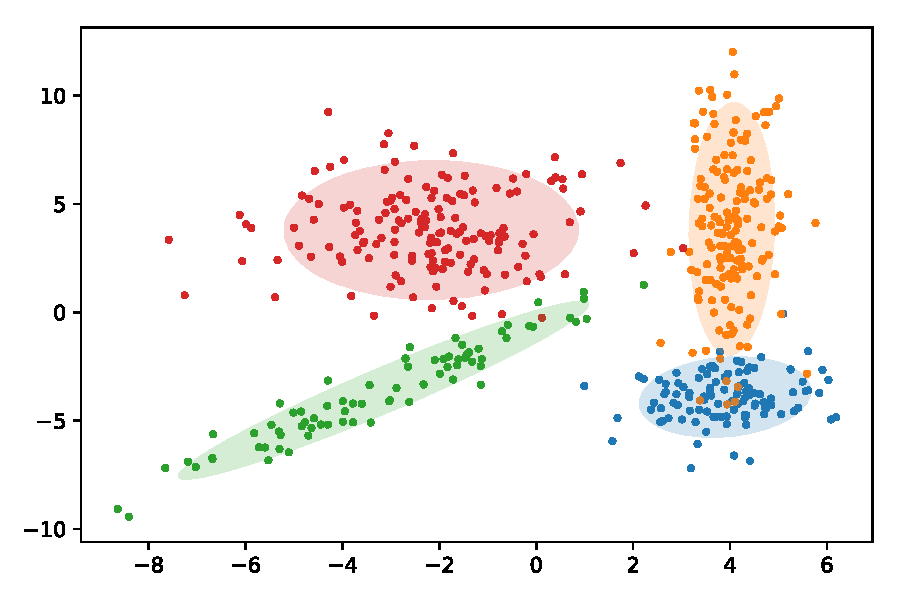
\includegraphics[width=0.7\textwidth]{clustering_viterbi.pdf}
    \caption{Most likely sequence of state returned by the Viterbi
      algorithm on the test data}\label{fig:clustering-viterbi}
  \end{figure}

\end{question}

\begin{question}
  The marginal probabilities $\pcond{q_t = i}{u_0, \dots u_T}$ for
  each state $i$ in $\intn{0}{3}$ are given in the figure
  \ref{fig:filtering-test}.

  \begin{figure}[h!]
    \centering
    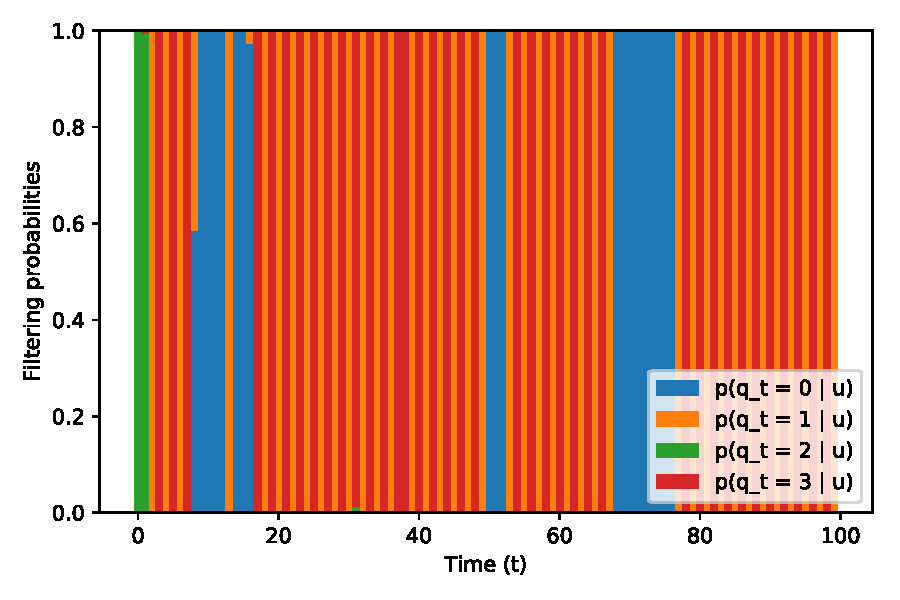
\includegraphics[width=0.7\textwidth]{filtering_test.pdf}
    \caption{Representation of the filtering probabilities
      $\pcond{q_t}{u_0, \dots u_T}$ for each state for the HMM trained
      on the test dataset}\label{fig:filtering-test}
  \end{figure}

  % \begin{figure}[p]
  %   \centering
  %   \begin{subfigure}[t]{0.48\textwidth}
  %     \centering
  %     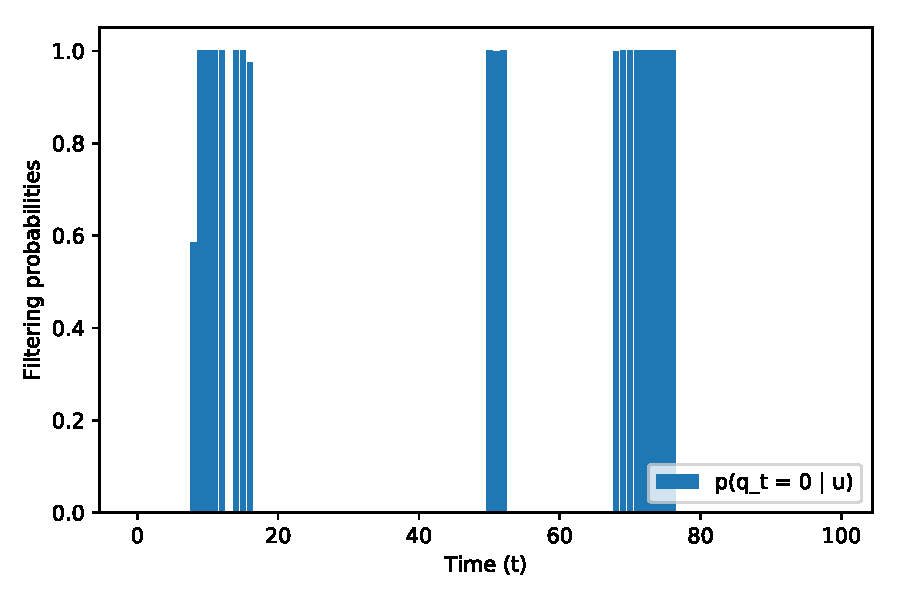
\includegraphics[width=\textwidth]{prediction_0.pdf}
  %     \caption{Training observations A ($150$ points)}\label{fig:LDA-A-train}
  %   \end{subfigure}
  %   \quad
  %   \begin{subfigure}[t]{0.48\textwidth}
  %     \centering
  %     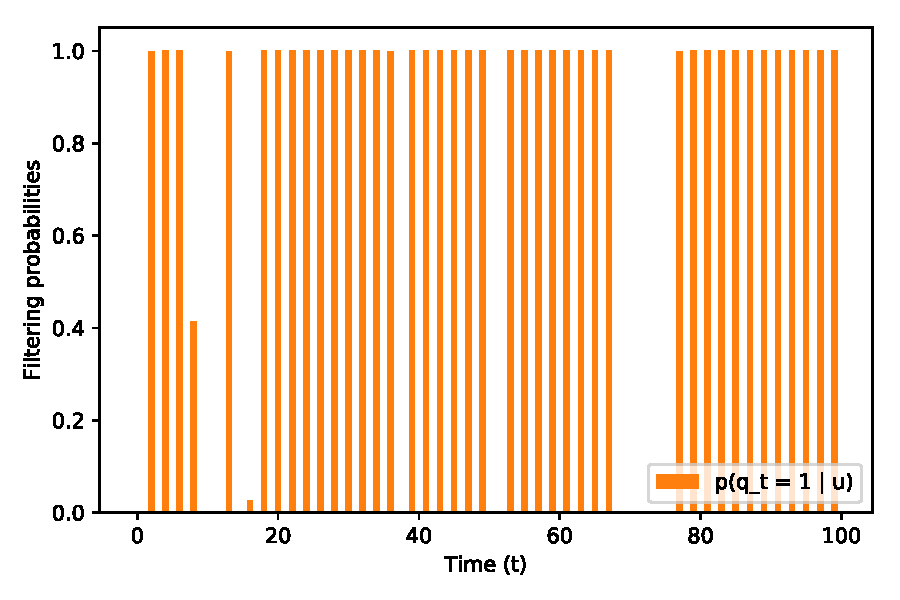
\includegraphics[width=\textwidth]{prediction_1.pdf}
  %     \caption{Test observations A ($1500$ points)}\label{fig:LDA-A-test}
  %   \end{subfigure}
  %   \vskip\baselineskip
  %   \begin{subfigure}[t]{0.48\textwidth}
  %     \centering
  %     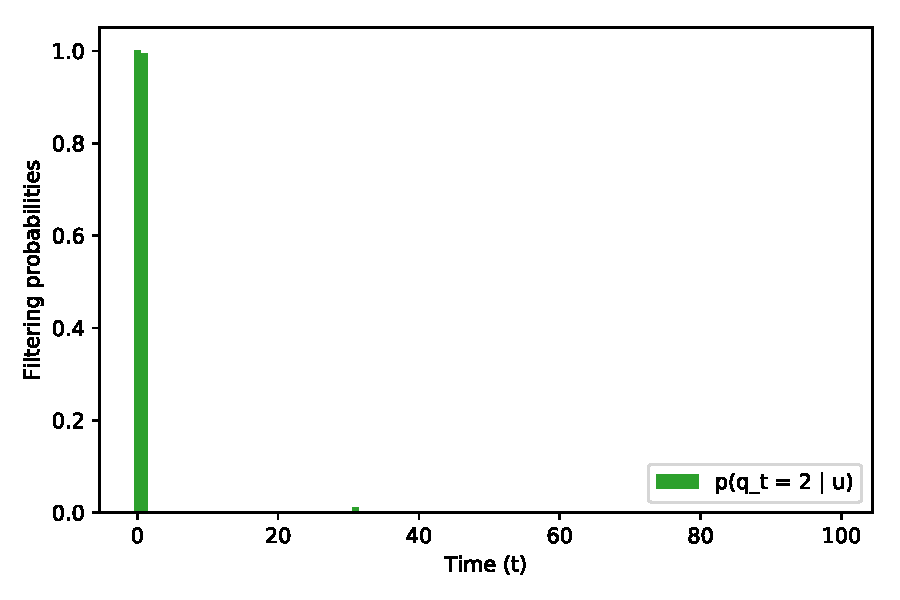
\includegraphics[width=\textwidth]{prediction_2.pdf}
  %     \caption{Training observations B ($150$ points)}\label{fig:LDA-B-train}
  %   \end{subfigure}
  %   \quad
  %   \begin{subfigure}[t]{0.48\textwidth}
  %     \centering
  %     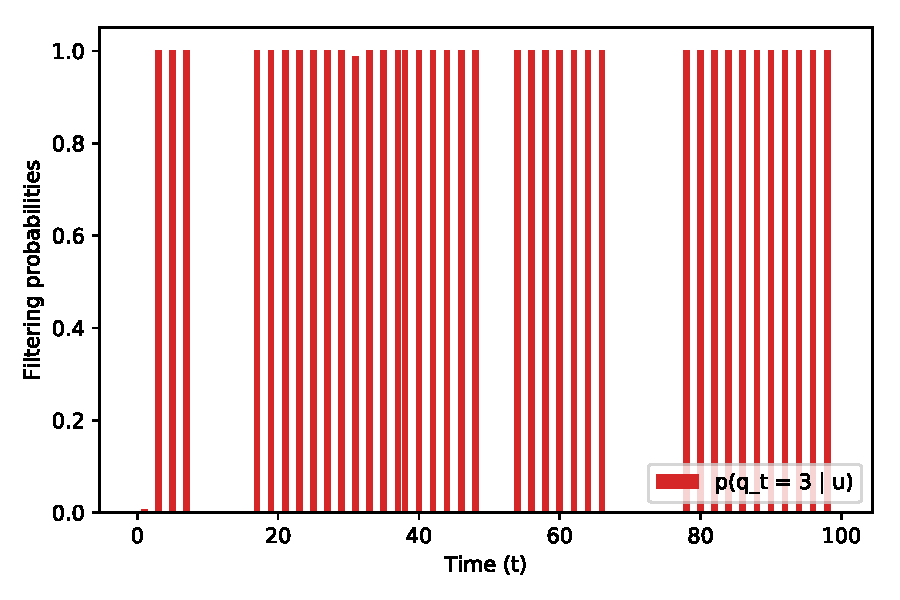
\includegraphics[width=\textwidth]{prediction_3.pdf}
  %     \caption{Test observations B ($1500$ points)}\label{fig:LDA-B-test}
  %   \end{subfigure}
  %   \caption{Sample data and decision boundary representation for the LDA classifier on the three files}\label{fig:LDA}
  % \end{figure}

\end{question}

\newpage
\begin{question}
  The most likely state of each datapoint according to the marginal
  probability $\pcond{q_t}{u_0, \dots u_T}$ of state is represented in
  figure \ref{fig:clustering-marginal}.

  \begin{figure}[h!]
    \centering
    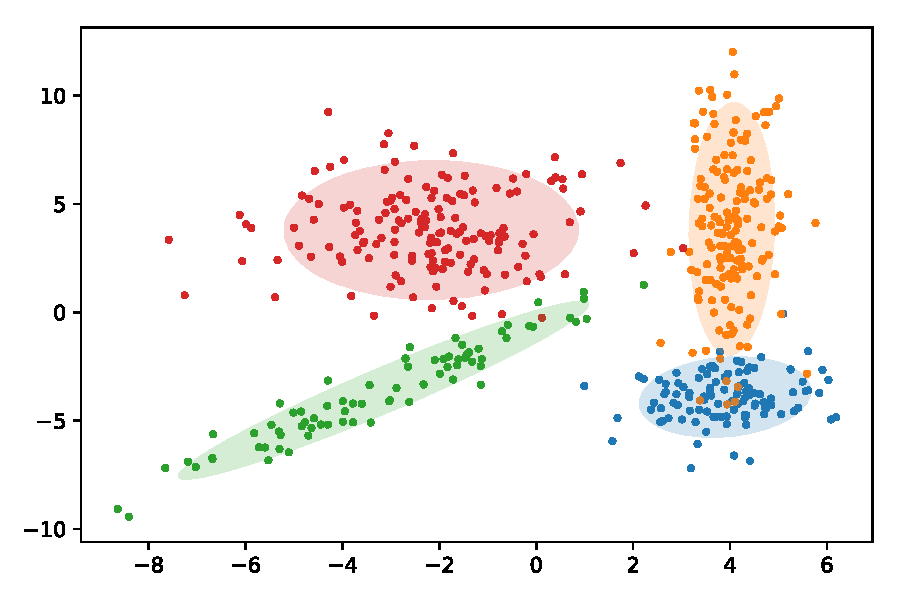
\includegraphics[width=0.7\textwidth]{clustering_marginal.pdf}
    \caption{Representation of the most likely state of each datapoint
      according to the marginal
      $\pcond{q_t}{u_0, \dots u_T}$}\label{fig:clustering-marginal}
  \end{figure}

\end{question}

\begin{question}
  The figure \ref{fig:classes-comparison} compares the most likely
  state for each datapoint according to both criterion (Viterbi and
  marginal probabilities). We see that there is no difference in this
  case (every point is assigned the same class). This means that this
  assignation of the point maximize both $p(q_t | u_0, \dots u_T)$ for
  all $t$ and $p(q_0, \dots, q_T | u_0, \dots u_T)$, put in word, the
  assignation of points corresponding to the most probable sequence of
  states also maximises the probability of each individual state. This
  shows that the trained model fits the data very well.

  % If the transition
  % probability are independant of the state, this is the case,


  % By taking the
  % most probable sequence, we expect to do sacrifices on the marginal
  % probability of each individual point, but in this particular case,
  % each assigned state also has maximal probability for its
  % corresponding point.

  \begin{figure}[p]
    \centering
    \begin{subfigure}[t]{0.70\textwidth}
      \centering
      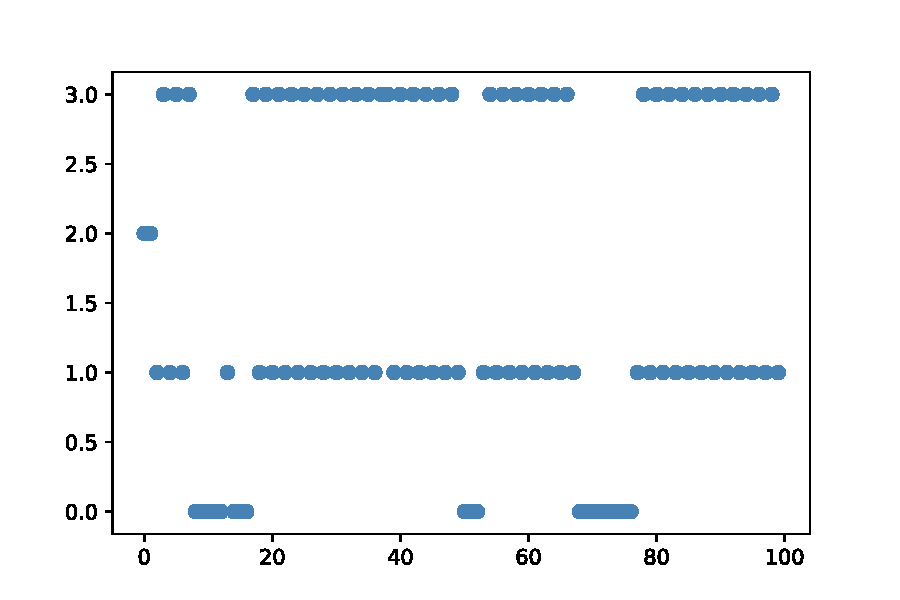
\includegraphics[width=\textwidth]{classes_viterbi.pdf}
      \caption{Most likely state for each datapoint according to the
        Viterbi criterion}\label{fig:classes-viterbi}
    \end{subfigure}
    \\
    \begin{subfigure}[t]{0.70\textwidth}
      \centering
      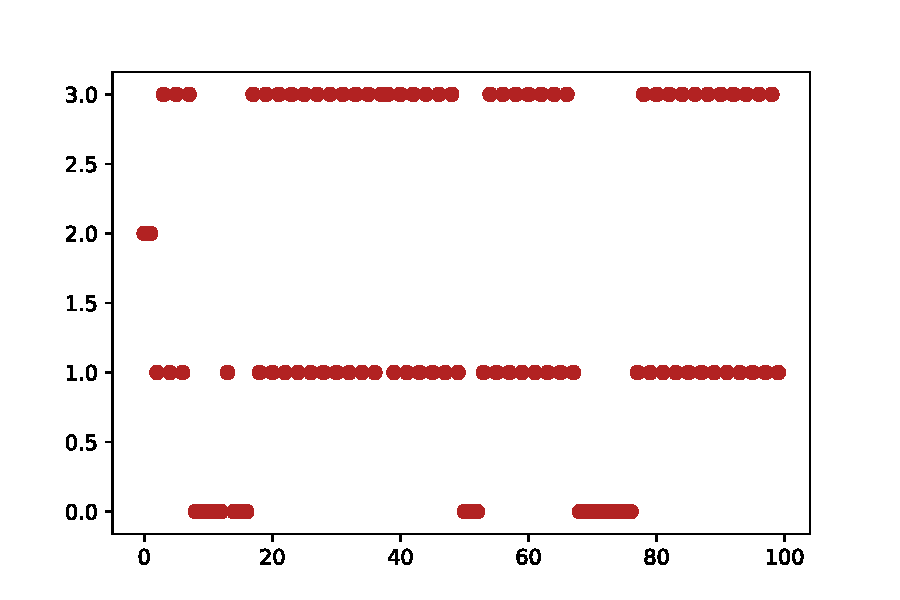
\includegraphics[width=\textwidth]{classes_marginal.pdf}
      \caption{Most likely state for each datapoint accordint to the
        marginal probability criterion}\label{fig:classes-marginal}
    \end{subfigure}
    \caption{Representation of the most likely states for each
      datapoint according to the Viterbi and the marginal probability
      criterion }\label{fig:classes-comparison}
  \end{figure}

\end{question}

\begin{question}
  As we increase the number of state, the likelihood will increase, we
  would like to maximize the likelihood but at the same time, we don't
  want the number of states to be too high, because it would lead to
  overfitting, and also impact the performances (the alpha beta
  recursion which is necessary for EM has a complexity of $O(S^2 T)$
  where $S$ is the number of states and $T$ the number of points, and
  the Viterbi algorithm also has the same complexity). As suggested in
  the lesson for K-means, we can have optimize a function of the
  number of states that recompense the likelihood of the model and
  penalize the number of states. There exist several model selection
  criterion based on this such as the Bayesian information criterion,
  which aims to
  \begin{equation*}
    \begin{aligned}
      & \underset{S}{\text{minimize}}
      & & \ln(T) S - 2 \ln(\mathcal{L}) \\
    \end{aligned}
  \end{equation*}
  To choose the number of state, one could increase the number of
  state up to the point where the gain in the likelihood factor do not
  compensate the cost of the number of state.

\end{question}

\end{document}

% \begin{figure}[h!]
%   \centering
%   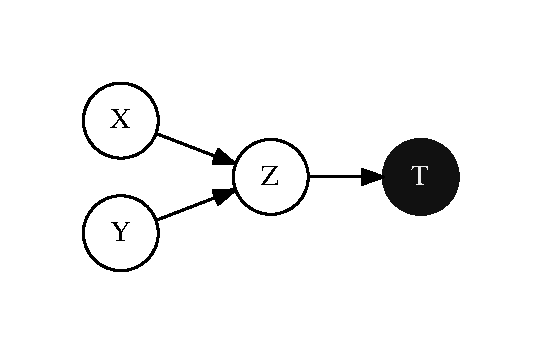
\includegraphics[width=0.5\textwidth]{graph.pdf}
%   \caption{Representation of Bayes ball algorithm on Graph G to
%     determine if $X$ and $Y$ are conditionally independant given
%     $T$}\label{fig:LDA-A-train}
% \end{figure}


%% \begin{figure}[p]
%%   \centering
%%   \begin{subfigure}[t]{0.40\textwidth}
%%     \centering
%%     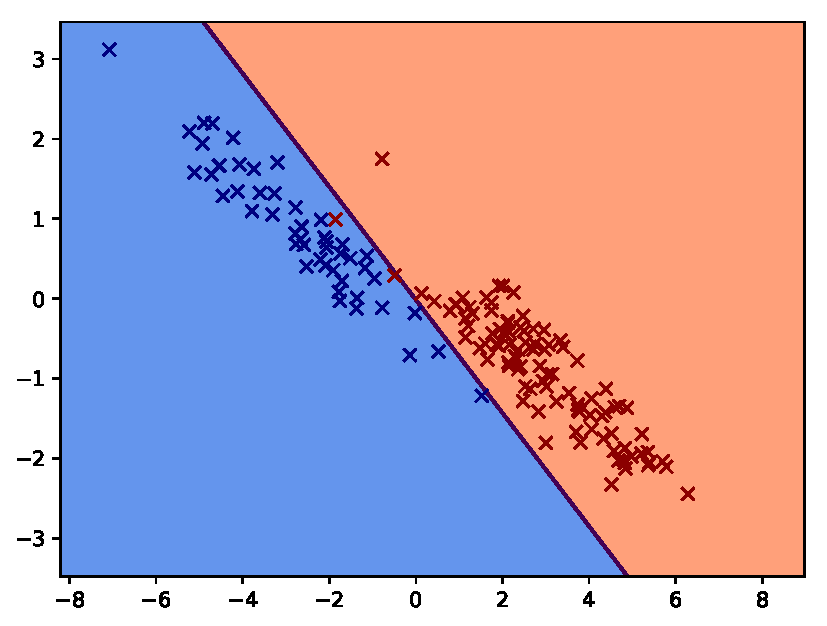
\includegraphics[width=\textwidth]{LDA_classificationA_train.pdf}
%%     \caption{Training observations A ($150$ points)}\label{fig:LDA-A-train}
%%   \end{subfigure}
%%   \quad
%%   \begin{subfigure}[t]{0.40\textwidth}
%%     \centering
%%     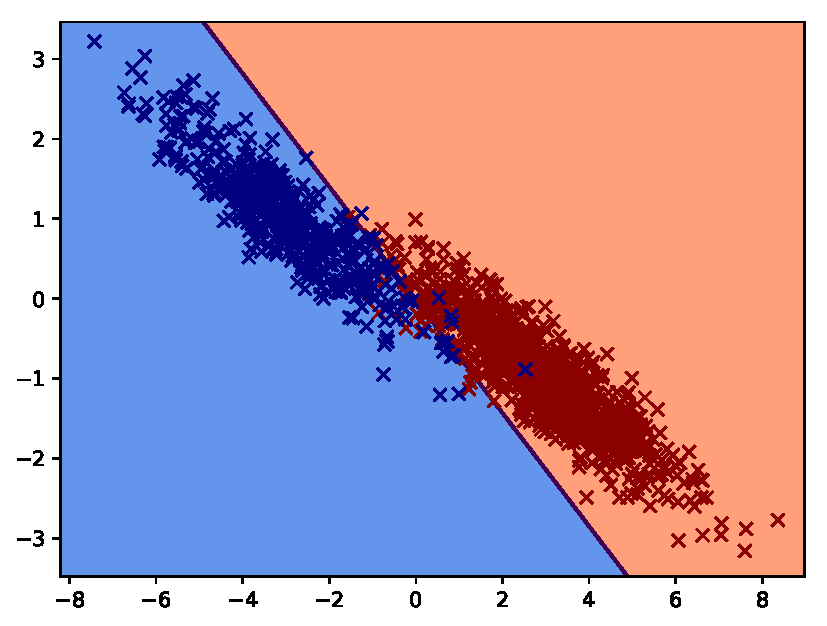
\includegraphics[width=\textwidth]{LDA_classificationA_test.pdf}
%%     \caption{Test observations A ($1500$ points)}\label{fig:LDA-A-test}
%%   \end{subfigure}
%%   \vskip\baselineskip
%%   \begin{subfigure}[t]{0.40\textwidth}
%%     \centering
%%     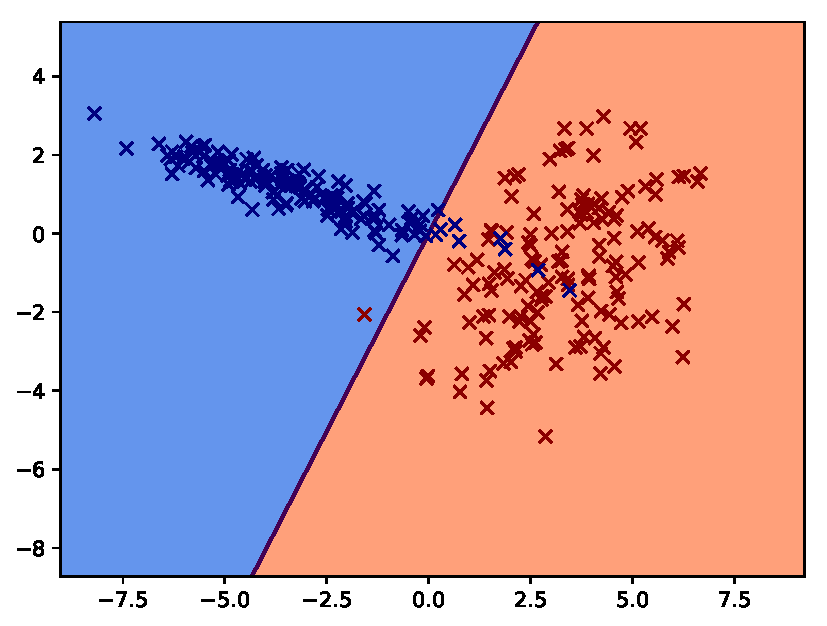
\includegraphics[width=\textwidth]{LDA_classificationB_train.pdf}
%%     \caption{Training observations B ($150$ points)}\label{fig:LDA-B-train}
%%   \end{subfigure}
%%   \quad
%%   \begin{subfigure}[t]{0.40\textwidth}
%%     \centering
%%     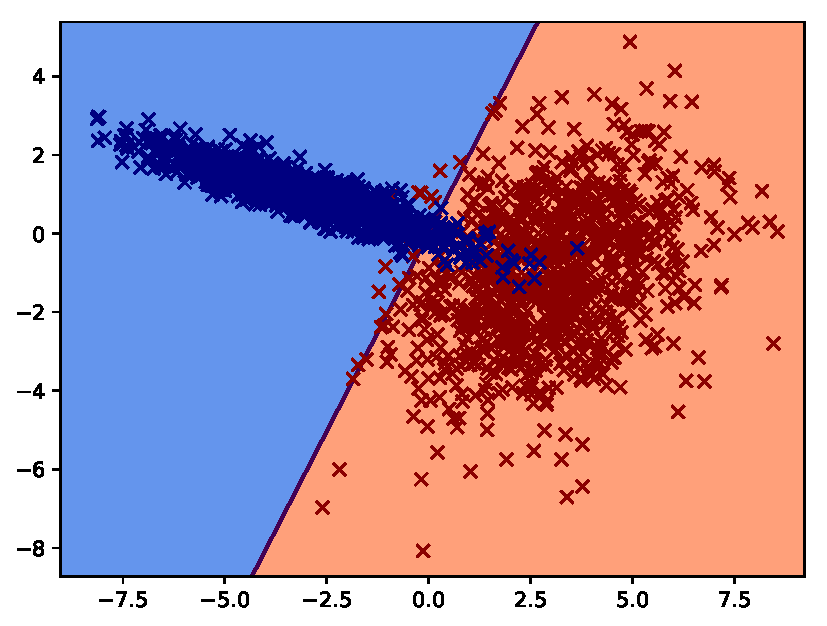
\includegraphics[width=\textwidth]{LDA_classificationB_test.pdf}
%%     \caption{Test observations B ($1500$ points)}\label{fig:LDA-B-test}
%%   \end{subfigure}
%%   \vskip\baselineskip
%%   \begin{subfigure}[t]{0.40\textwidth}
%%     \centering
%%     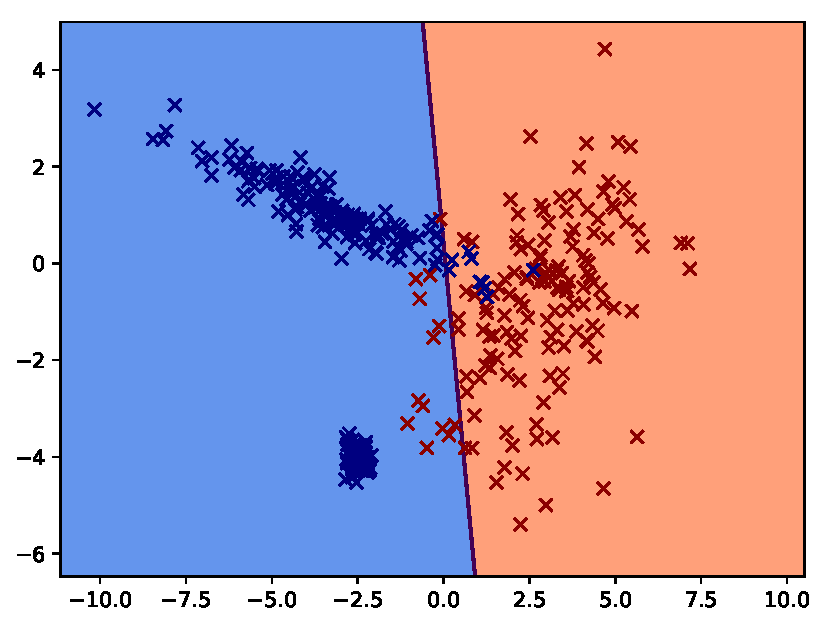
\includegraphics[width=\textwidth]{LDA_classificationC_train.pdf}
%%     \caption{Training observations C ($150$ points)}\label{fig:LDA-C-train}
%%   \end{subfigure}
%%   \quad
%%   \begin{subfigure}[t]{0.40\textwidth}
%%     \centering
%%     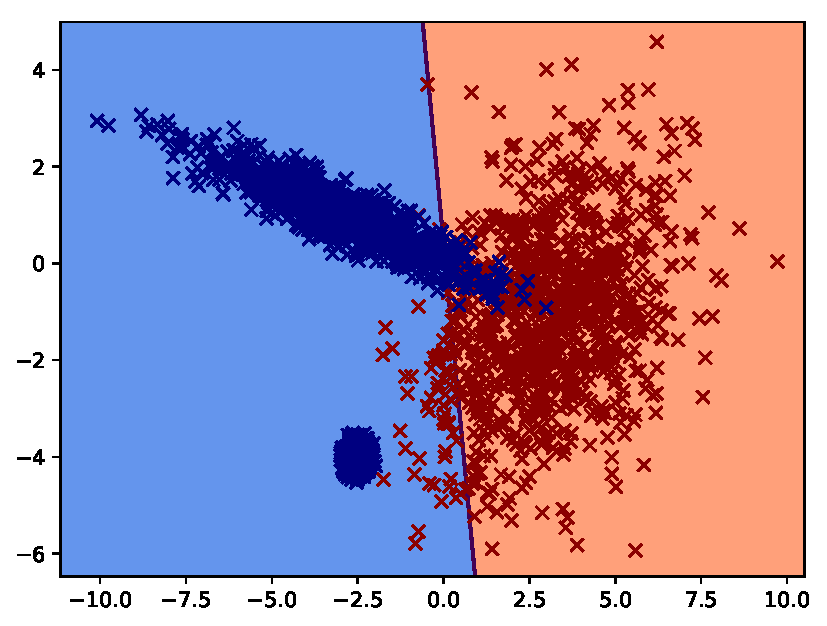
\includegraphics[width=\textwidth]{LDA_classificationC_test.pdf}
%%     \caption{Test observations C ($1500$ points)}\label{fig:LDA-C-test}
%%   \end{subfigure}
%%   \caption{Sample data and decision boundary representation for the LDA classifier on the three files}\label{fig:LDA}
%% \end{figure}


% \begin{figure}[h!]
%   \centering
%   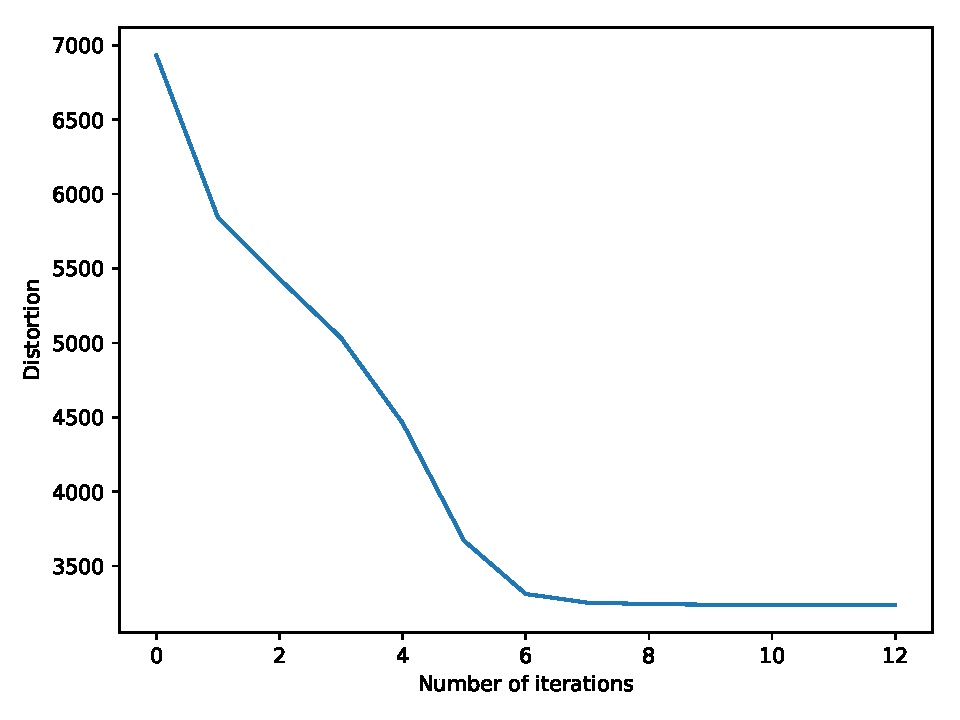
\includegraphics[width=0.6\textwidth]{kmeans4_distortion.pdf}
%   \caption{Evolution of the distortion with respect to the number of
%     iterations for an execution of the Kmeans algorithm}\label{fig:kmeans4-distortion}
% \end{figure}

% \begin{figure}[h!]
%   \centering
%   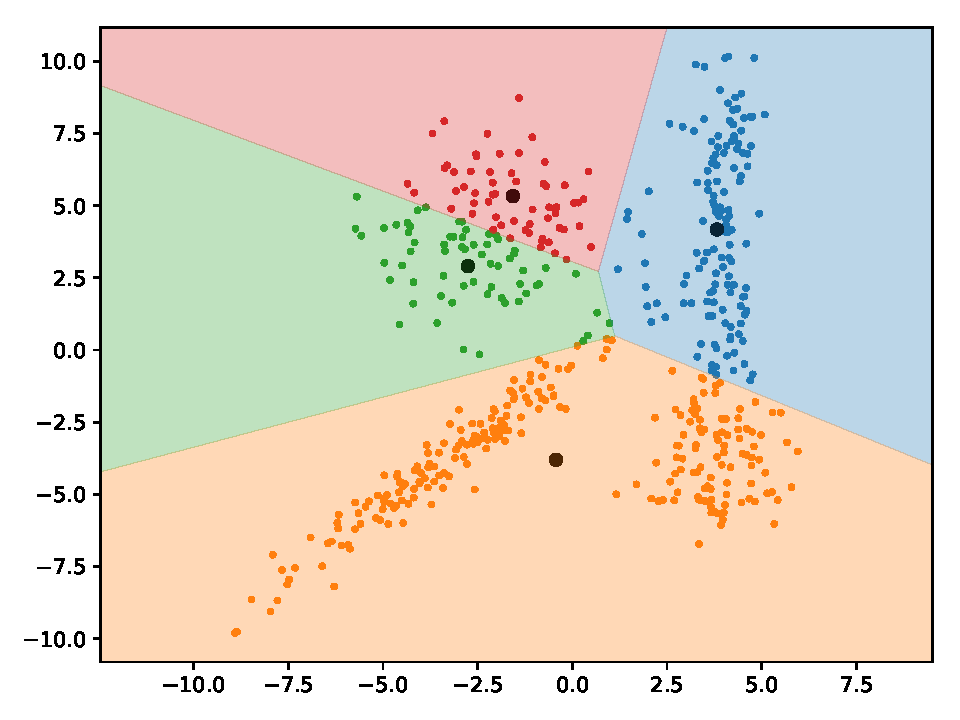
\includegraphics[width=0.7\textwidth]{kmeans4_failure.pdf}
%   \caption{Representation of the training points, the means returned
%     by an execution of the K-means algorithm ($K = 4$) that has
%     converged to a bad local minimum (distortion =
%     6378.84, convergence in 5
%     iterations)}\label{fig:kmeans4-failure}
% \end{figure}

%% \begin{table}[h!]
%%   \centering
%%   \begin{tabular}{| l | l | l | l | c | c |}
%%     \hline
%%     sample file & $\pi$ & $\mu_0$ & $\mu_1$ & $\Sigma_0$ & $\Sigma_1$ \\
%%     \hline
%%     \file{classificationA} &
%%     0.33 & ( 2.90, -0.89 ) & ( -2.69, 0.87  ) &
%%     \( \left( \begin{array}{cc}
%%       2.33 & -1.06 \\
%%       -1.06 &  0.58
%%     \end{array} \right) \) &
%%     \( \left( \begin{array}{cc}
%%       2.76 & -1.33 \\
%%       -1.33 &  0.70 \\
%%     \end{array} \right) \) \\

%%     \file{classificationB} &
%%     0.5 & ( 3.34, -0.84 ) & ( -3.22, 1.08) &
%%     \( \left( \begin{array}{cc}
%%       2.56 &  1.07 \\
%%       1.07 &  2.98 \\
%%     \end{array} \right)  \) &
%%     \( \left( \begin{array}{cc}
%%       4.18 & -1.34 \\
%%       -1.34 &  0.52 \\
%%     \end{array} \right)  \) \\

%%     \file{classificationC} &
%%     0.625 & ( 2.79, -0.84 ) & ( -2.94,-0.96 ) &
%%     \( \left( \begin{array}{cc}
%%       2.92 &  1.25 \\
%%       1.25 &  2.94  \\
%%     \end{array} \right)  \) &
%%     \( \left( \begin{array}{cc}
%%       2.88 &  -1.77 \\
%%       -1.77 &  6.59 \\
%%     \end{array} \right)  \) \\
%%     \hline
%%   \end{tabular}
%%   \captionof{table}{Parameters learnt for the QDA method for the different training sample} \label{tab:ParamQDA}
%% \end{table}
